La distribuci\'on normal es una de las distribuciones que mas aparece en la vida real. A continuaci\'on se presentan 2 ejemplos de la misma.
	
	\subsubsection*{Altura de una persona}
	
		Es ampliamente conocido que las caracter\'isticas morfol\'ogicas de individuos, tales como la estatura, siguen el modelo normal en todo el mundo. En general, se puede pensar la altura de las personas suele estar entre 1-70 y 1.75 metros, debido a que en la mayor\'ia de los casos es as\'i. Es minor\'ia las personas que midan menos de 1.50, y a la vez no hay tampoco demasiadas personas que superen los 2 metros. Haciendo un muestreo poblacional y realizando un histograma del mismo se puede visualizar esta intuici\'on.
		
\begin{figure}[H]
  \begin{center}
    %\includegraphics[scale=.41,angle=-90]{imgenes/normal_ejemplo1.png}
    \includegraphics[scale=.40]{imagenes/normal_ejemplo1.png}
    \caption{Histograma altura} 
    \label{fig:normal_ejemplo1}
  \end{center}
\end{figure}		
		
Se puede ver como para el muestreo realizado, la mayor\'a de las personas caen en la altura entre 1.70 y 1.80 metros, dando como resultado aproximadamente, una normal con media 1,75 y desv\'io standard 0.64.

\newpage

	\subsubsection*{IQ de una persona}
	
		Otro ejemplo muy conocido es el coeficiente intelectual de las personas, conocido como IQ. Seg\'un el siguiente ranking, vemos que una inteligencia normal deber\'ia estar entre los 90 y los 109 de coeficiente intelectual. Por lo que es de esperar que la mayor parte de la poblaci\'on este en este promedio.
\newline

\begin{tabular}{| l | l |}
\hline
IQ Range & Clasificaci\'on \\
\hline
130 o mas & Muy Superior \\
\hline
120\--129	& Superior \\
\hline
110\--119	& Arriba del promedio \\
\hline
90\--109	& Promedio \\
\hline
80\--89	& Abajo del Promedio \\
\hline
70\--79	& L\'imite \\
\hline
69 o menos & Extremadamente bajo \\
\hline
\end{tabular}
\newline

\noindent 
Veamos un histograma sobre el muestreo del IQ de los individuos de una poblaci\'on. 


\begin{figure}[H]
  \begin{center}
    %\includegraphics[scale=.41,angle=-90]{imgenes/normal_ejemplo1.png}
    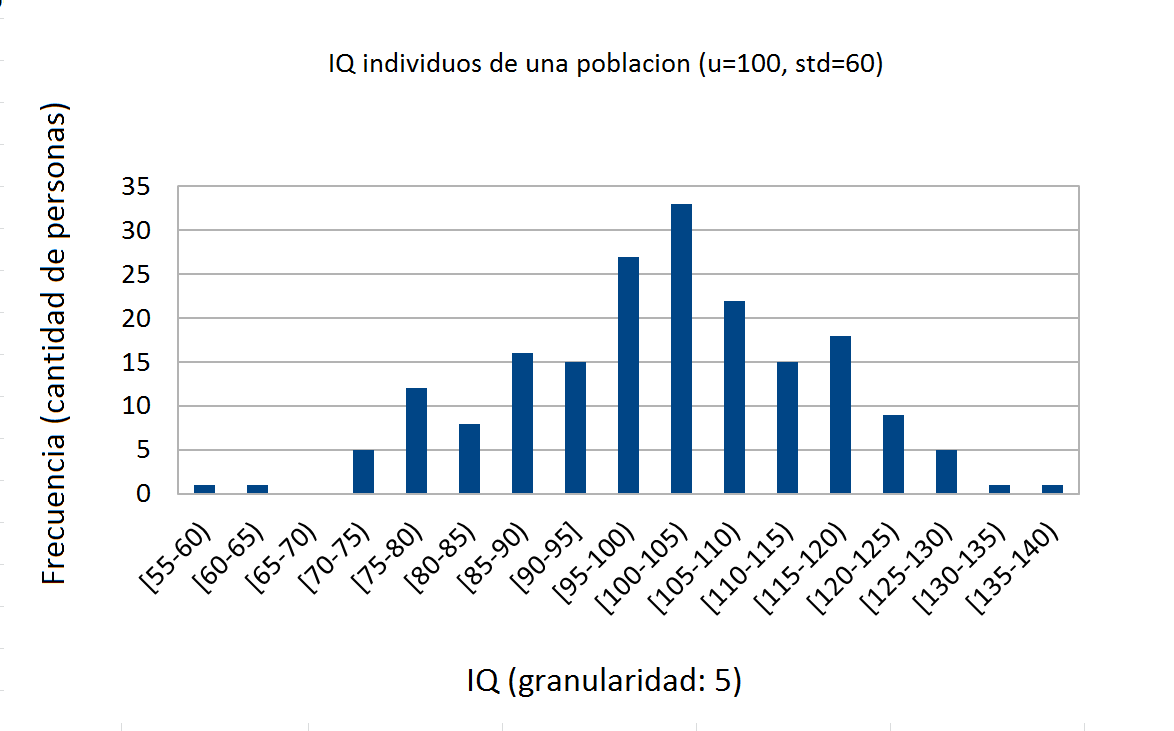
\includegraphics[scale=.40]{imagenes/normal_ejemplo2.png}
    \caption{Histograma IQ} 
    \label{fig:normal_ejemplo2}
  \end{center}
\end{figure}	

En la figura \ref{fig:normal_ejemplo2}, podemos un ver como, efectivamente, la mayor\'ia de la poblaci\'on se centra en un IQ de 100, con una desv\'io al rededor de 20.